\documentclass[11pt]{report}

% French packages
\usepackage[utf8]{inputenc}
\usepackage[T1]{fontenc}
\usepackage[francais]{babel}

% Geometry
\usepackage[top=2cm, bottom=2cm, left=3cm, right=3cm]{geometry}

% Fonts
\usepackage{lmodern}

% Outline text
\usepackage{fancybox} 

% Custom colors
\usepackage{color}
    \definecolor{dkgreen}{rgb}{0,0.6,0}
    \definecolor{gray}{rgb}{0.5,0.5,0.5}
    \definecolor{mallow}{rgb}{0.58,0,0.82}

% Assets path
\usepackage{graphicx}
    \graphicspath{{./assets/}}

\usepackage{lipsum}

% Custom syntax highlighting
\usepackage{listings}
    \lstset{
        language=C++,
        aboveskip=3mm,
        belowskip=3mm,
        showstringspaces=false,
        columns=flexible,
        basicstyle={\small\ttfamily},
        numbers=none,
        numberstyle=\tiny\color{gray},
        keywordstyle=\color{blue},
        commentstyle=\color{dkgreen},
        stringstyle=\color{mallow},
        breaklines=true,
        breakatwhitespace=true,
        tabsize=4
    }

% Header/footer
\usepackage{fancyhdr}
    \fancypagestyle{utt}{
        \setlength{\headheight}{23.96pt}
        \fancyfoot[C]{\thepage}
        \fancyhead[L]{\leftmark{}}
        \fancyhead[R]{
\includegraphics[scale=1.5]{logo_utt.jpg}}

        % Rename table of contents
        \addto\captionsfrench{\renewcommand{\contentsname}{Sommaire}}
    }

    \pagestyle{utt}


\title{Rapport de projet NF05}
\author{Axel \bsc{Mousset} Aurélien \bsc{Labate} \\ Université de Technologie de Troyes}
\date{Automne 2014}


\begin{document}
    \maketitle
    \tableofcontents

    \chapter{Introduction}
    \lipsum[1-2]
    \chapter{Choix technologiques}
    \section{Language C++}
        La première étape dans ce projet a été de choisir le language dans lequel il serait développé: la contrainte qui nous était imposée 
        était le choix entre le language C et ses dérivés.
        \\ Le C est un language de programmation généraliste et bas niveau inventé dans les années 1970. C'est un des language les plus utilisé 
        au monde, pionnier du monde informatique, qui a inspiré nombre d'autre language et donné naissance à des dérivés comme le C\#\footnote{Prononcer ``C sharp''}, 
        l'Objective-C ou encore le C++.
        \\ Notre choix s'est porté sur ce dernier, car il intègre bon nombre de concepts plus récents en programmation comme la POO\footnote{Programmation
        orientée objet} qui nous sont familiers. Il n'est également d'aucune affiliation particulière avec les entreprises: le C\# étant développé par microsoft
        et l'objective-C par Apple.
        \\ Une fois le language choisi, nous nous sommes intéressés au différents frameworks\footnote{Espace de travail - sorte de grande bibliothèque 
        de programmation}
        graphiques disponibles.


    \section{Framework Qt}
        \begin{figure}[h]
            \begin{center}
                
\includegraphics[scale=0.3]{Qt.png}
            \end{center}

            \caption{Logo de Qt}
            \label{Qt}
        \end{figure}

        La motivation derrière l'utilisation de Qt résulte tout d'abord de la volonté d'avoir un programme multi-plateforme. Le développement du programme étant fait dans un environnement linux, et avec une majorité d'ordinateurs tournant sous windows, la nécessité d'avoir un programme portatif était évidente.
        \\ Un rapide tour d'horizon sur les différents frameworks/libraries multi-plateformes montre qu'il n'y a essentiellement que trois grand projet: WxWidgets, GTK et Qt.
        \\ L'avantage de Qt par rapport a ses concurrents est qu'il jouit d'une très large communauté, et est maintenu par Nokia. C'est un framework très moderne allant jusqu'à étendre le C++ pour lui apporter des fonctionnalités non natives. Il permet donc le développement dans un environnement plus haut niveau, au détriment des performances du programme, que nous avons jugées négligeables étant donnée l'échelle du programme.
        \\ Enfin, en plus de faciliter le développement du coeur du programme, Qt à l'avantage de proposer un IDE\footnote{Integrated development environment}, Qt Creator, qui dispose d'une auto-complétion très poussée ainsi qu'un éditeur WYSIWYG\footnote{What you see is what you get - il n'y a qu'à dessiner pour obtenir ce que l'ont veux} d'interface graphique.

        \begin{figure}[h]
            \begin{center}
                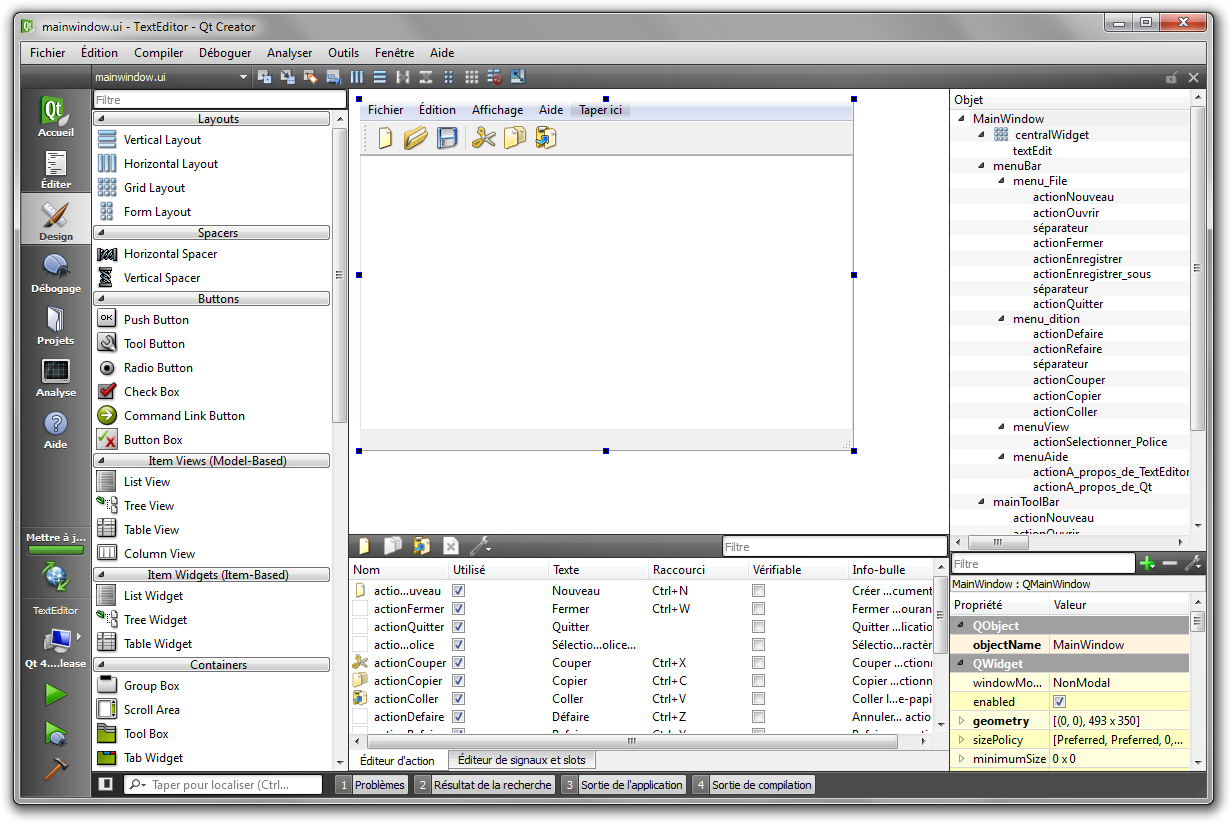
\includegraphics[scale=0.3]{Qt_creator.png}
            \end{center}

            \caption{Éditeur d'interface WYSIWYG de Qt Creator}
            \label{Qt Creator}
        \end{figure}

    \newpage

    \section{Gestionnaire de version et travail collaboratif Git}
        \paragraph{}
            Bien que n'étant qu'en binôme, travailler en équipe sur un même code sans outil approprié se révèle souvent être un enfer. En effet, la modification d'un fichier peut entrainer des incompatibilités et des bugs dans le reste du programme. Et c'est à ce genre de problèmes que vient répondre un gestionnaire de version.
            \\ Tout comme les frameworks graphiques, il existe plusieurs solutions sur le marché, on retiendra essentiellement svn et git. Le choix de git fût immédiat car maitrisé par l'ensemble de l'équipe. 
            \\ Git a été créé en 2005 par Linus Torvalds, créateur de noyau linux, devant la nécessité de cannaliser et organiser les contributions des milliers de contributeurs de linux. C'est le gestionnaire de version le plus utilisé, et est un réel standard dans le monde du développement logiciel.

        \paragraph{}
            Git est un outil déscentralisé, un service : il doit être herbergé par un serveur. Là ou il est possible d'être indépendant et d'héberger son propre serveur github, nous avons préferé nous rabattre sur un hébergeur gratuit et public, github.
            \\ Ce choix est motivé et par la facilité d'utilisation qu'offre github, mais aussi par la volonté d'avoir un programme libre. Github met ainsi à 
            disposition librement et pour tous notre programme, sous la licence de notre choix (ici MIT).
            
            \begin{figure}[h]
                \begin{center}
                    
\includegraphics[scale=0.3]{logo_github.jpg}
                \end{center}

                \caption{Logo de github}
                \label{github}
            \end{figure}

    \newpage


    \section{Générateur de documentation Doxygen}
        \lipsum[1-2]
    \chapter{Algorithmes utilisés}
    La recherche des algorithmes et leur développement fut l'un des gros morceaux du projet. Cette partie pris une semaine de développement.

    \section{Design pattern: Lexer/Parser}
        \begin{figure}[h]
            \begin{center}
                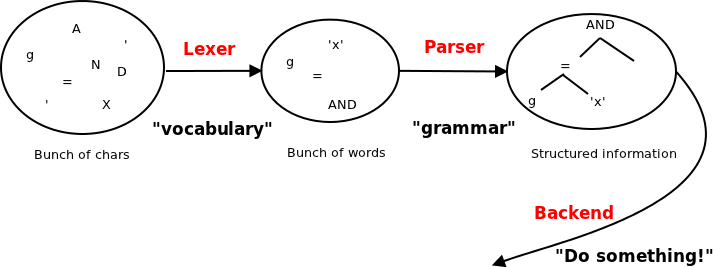
\includegraphics[scale=0.5]{lexer_parser.png}
            \end{center}

            \caption{Représentation du Lexer/Parser}
            \label{Représentation du Lexer/Parser}
        \end{figure}

        \paragraph{}
            Le choix a été fait de remplir un des objectifs secondaires du cahier des charges, ``l'imbrication libre des instructions''.
            \\ Le problème a été traité de manière traditionnelle, une utilisant le design pattern lexer/Parser.
            \\ Le lexer, est ``l'analyseur lexical''. Il transforme une série de caractères en ``tokens'', qui sont des chaînes de caractères définies au préalable.
            \\ Ainsi, un mot est un token ``T\_STRING'', un chiffre est un token ``T\_SCALAR'' ou encore une matrice un ``T\_MATRIX''. Au niveau du code, ces tokens sont représentés par des objets (voir \ref{lib/token.h}) ayant chacun la valeur de la chaine de caractère reconnue associée à leur type. Exemple : le chiffre 3 est un objet Token de type ``T\_SCALAR'' et de valeur ``3''.
            \\ La reconnaissance de ces tokens se fait par regex successive sur la chaine de caractère ce que l'une d'entre elle fonctionne.
      
            \begin{figure}[h]
                \begin{center}
                    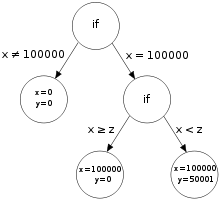
\includegraphics[scale=1]{syntax_tree.png}
                \end{center}

                \caption{Création d'un arbre d'execution. Des noeuds conditionnels sont représentés}
                \label{Représentation arbre syntaxique}
            \end{figure}

        \newpage

        \paragraph{}
            Une fois l'expression analysée, il faut l'exécuter. Le parser passe en revue tous les tokens en essayant de reconnaître des ``motifs'' d'expression cohérentes. Il les assemble ensuite en Node (voir \ref{lib/node.h}), qui sont comme leur nom l'indique des noeuds d'expression. Un exemple de noeud est le noeud d'assignation, ayant comme motif un nom de variable et une expression séparée par un signe égal.


            Le code est pensé de manière modulaire, il est ainsi possible de rajouter d'autres types de noeud comme des noeuds conditionnels par exemple, et ainsi étendre l'analyseur d'expression en un véritable interpréteur de language.
            \\ Les Nodes créées, elles sont ensuite assemblées en arbre et ensuite exécutée. Nous allons maintenant voir par quelle méthode les  expressions sont interprétées.

    \section{Execution des expression: Notation Polonaise Inversée}
        L'execution des expressions peut se faire de plusieurs manières. La première qui a été abordée puis abandonnée par la suite, est la création d'un arbre syntaxique similaire à l'arbre d'éxecution introduit à la section précédente. Le problème avec cette manière de fonctionner est qu'elle est bien plus lourde niveau code et donc source de bugs. Une implémentation de cette méthode a néammoins été produite et reste visible dans l'historique des commits du projet.
        \\ L'autre manière d'aborder le problème et qui a été retenue pour le projet est la conversion de l'expression sous sa forme infixe (forme usuelle, utilisant les parenthèses) en notation polonaise inversée, une forme d'expression bien plus simple a exécuter qui ne comprend ni parenthèses ni priorité d'opérateurs.
        \\ Voici un exemple simple d'expression.
        \begin{equation}
            (2 + 4) * 2
        \end{equation}
        Une fois convertis en notation polonaise inversée, celà donne l'expression suivante.
        \begin{equation}
            2 4 + 2 *
        \end{equation}
        Le principe est d'empiler opérandes et opérateurs, chaque opérateurs opérant sur les deux opérandes qui le précède.
        \\ Cette méthode, très connue et largement utilisée par les compilateurs nous a permis de trouver une implémentation de l'algorithme permettant la conversion de l'expression, et quant à l'éxecution de l'expression, c'est un jeux d'enfant.
    \chapter{Fonctionnement du programme}
    \section{Interface graphique}
        \begin{figure}[h]
            \begin{center}
                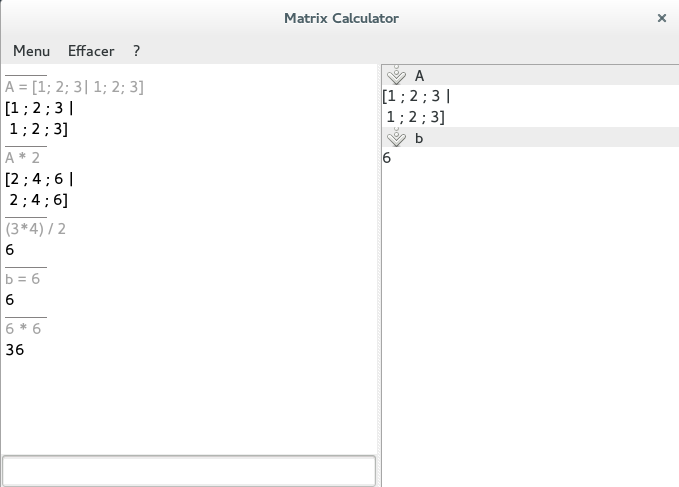
\includegraphics[scale=0.5]{interface.png}
            \end{center}

            \caption{Interface du programme}
            \label{Interface du programme}
        \end{figure}

    L'interface est composée d'un champ d'entrée de sélection, d'une zone d'affichage comprenant les expressions entrées et leurs résultat (ou erreur) ainsi qu'une gestionnaire de variable.
    \\ Dans la partie principale, l'expression entrée par l'utilisateur est en gris et les erreurs, s'il y en a, sont affichées en rouges. et le resultat retournée par son expression en noir. Chaque expression est séparée par une ligne noire.
    \\ Il est possible à l'aide des flèches de remonter ou redescendre dans l'historique des entrées, en ayant pris soin de sélectionner la zone de texte d'entrée.
 

    \newpage

    \section{Fonctionnalités}
        \paragraph{}
            Les variables et leur contenu sont affichés en temps réel sur la droite. L'utilisateur peut vider le contenu des variables en cliquant droit sur l'une d'elle, un menu contextuel apparaît et offre la possibilité de la supprimer.
            \\ En cliquant simplement sur le nom de la variable, il est possible d'afficher ou de cacher sont contenu.
            \\ La suppression des variables, ainsi que celle de l'historique est disponible dans le menu ``effacer''.

        \paragraph{}
            L'état actuel du programme (contenu des variables ainsi qu'historique des entrées) peut être sauvegardé dans un fichier à l'aide du raccourcis clavier Ctrl+S ou dans le menu ``Menu''.
            \\ De la même manière, un état précédent du programme peut être récuperé en ouvrant un fichier avec le raccourcis Ctrl+O ou dans le menu ``Menu''.

        \paragraph{}
            Les opérateurs mathématiques de bases sont utilisables, à savoir la multiplication et la division, la somme et la différence, et la puissance (de caractères réspectifs * / + - et ^).
            \\L'assignation à une variable se fait de la manière suivante: \[nomVariable = [valeur]\] 
            \\ La valeur peut être un scalaire, la résultante d'une fonction ou une matrice.
            \\ Les fonctions implémentées sont :
            \begin{enumerate}
                \item Le déterminant d'une matrice \[det([matrice])\]
                \item L'inverse d'une matrice \[inv([matrice])\]
                \item La résolution d'équation linéaires (scalaires ou matricielles): \[solve([A], [B])\] 
                \item La création de matrice identitée \[I([taille])\]
                \item Le cofacteur d'une matrice \[cof([matrice])\]
                \item La comatrice d'une matrice \[co([matrice])\]
                \item La transposée d'une matrice \[trans([matrice])\]
                \item La norme d'une matrice \[norm([matrice])\]
            \end{enumerate}
            La syntaxe de définition d'une matrice est la suivante (pour une matrice 2x2)
                \[ [ [valeur]; [valeur] | [valeur]; [valeur] ]\]
            Le ``;'' est le séparateur de colonne et ``|'' le séparateur de ligne.

    \chapter{Conclusion}
   \lipsum[1-2]

    \appendix
    \chapter{Annexes}
    \section{Code}
      %  \lstinputlisting[language=C++]{../sources/mainwindow.cpp}
\lstinputlisting[language=C++]{../sources/detailedlist.cpp}
\lstinputlisting[language=C++]{../sources/mainwindow.hpp}
\lstinputlisting[language=C++]{../sources/about.cpp}
\lstinputlisting[language=C++]{../sources/detailedlist.hpp}
\lstinputlisting[language=C++]{../sources/about.h}
\lstinputlisting[language=C++]{../sources/main.cpp}
\lstinputlisting[language=C++]{../sources/lib/token.h}
\lstinputlisting[language=C++]{../sources/lib/calculables/matrix.cpp}
\lstinputlisting[language=C++]{../sources/lib/calculables/scalar.h}
\lstinputlisting[language=C++]{../sources/lib/calculables/matrix.h}
\lstinputlisting[language=C++]{../sources/lib/calculables/scalar.cpp}
\lstinputlisting[language=C++]{../sources/lib/assignationNode.cpp}
\lstinputlisting[language=C++]{../sources/lib/varNode.cpp}
\lstinputlisting[language=C++]{../sources/lib/calculable.h}
\lstinputlisting[language=C++]{../sources/lib/lexer.cpp}
\lstinputlisting[language=C++]{../sources/lib/node.h}
\lstinputlisting[language=C++]{../sources/lib/calculable.cpp}
\lstinputlisting[language=C++]{../sources/lib/parser.cpp}
\lstinputlisting[language=C++]{../sources/lib/token.cpp}
\lstinputlisting[language=C++]{../sources/lib/operator.h}
\lstinputlisting[language=C++]{../sources/lib/parser.h}
\lstinputlisting[language=C++]{../sources/lib/expressionNode.cpp}
\lstinputlisting[language=C++]{../sources/lib/operator.cpp}
\lstinputlisting[language=C++]{../sources/lib/assignationNode.h}
\lstinputlisting[language=C++]{../sources/lib/expressionNode.h}
\lstinputlisting[language=C++]{../sources/lib/varNode.h}
\lstinputlisting[language=C++]{../sources/lib/lexer.h}
\lstinputlisting[language=C++]{../sources/lib/node.cpp}
 to include all source codes

\end{document}